\begin{parts}

\part[2] Which of the following are convex? \textbf{Select all that apply:}
    \checkboxchar{$\Box$}
    \begin{checkboxes}
     \choice $f(x) = \max(0,x)$
     \choice $f(x) = \frac{53}{6}x + 42$
     \choice $f(x) = \log(1 + e^x)$
     \choice $f(x) = \sin(x)$
     \choice $f(x) = \|\xv\|_2^2$
    \end{checkboxes}
    \begin{soln}
  %  A,B,C,E. 
    \end{soln}


\part[1] \textbf{True or False:} Consider training a decision tree to learn a classification function $f: X \rightarrow \{-1, +1\}$ where each instance $x$ is defined by $n$ binary features ($x = <x_1 \ldots x_n>$, $x_i \in \{-1, 1\}$).  In this case, the decision tree can achieve zero training error for any noise-free training data set (i.e., for any training data set that doesn't contain two copies of the same $x$, one labeled 1 and the other labeled -1) {\em using a tree whose depth is at most $n-2$}.
    \begin{checkboxes}
     \choice True 
     \choice False
    \end{checkboxes}
    \begin{soln}
  %  False
    \end{soln}
    \begin{qauthor}
    Tom
    \end{qauthor}
    
\part[1] \textbf{True or False:} Consider training a decision tree to learn a classification function $f: X \rightarrow \{-1, +1\}$ where each instance $x$ is defined by $n$ binary features ($x = <x_1 \ldots x_n>$, $x_i \in \{-1, +1\}$).  In this case, the decision tree can achieve zero training error for any noise-free training data set (i.e., for any training data set that doesn't contain two copies of the same $x$, one labeled 1 and the other labeled -1).
    \begin{checkboxes}
     \choice True 
     \choice False
    \end{checkboxes}
    \begin{soln}
  %  True
    \end{soln}
    \begin{qauthor}
    Tom
    \end{qauthor}
    
\part[4] Consider how the above overfitting plot would change if we double the number of training examples.  How do you expect this plot to change? \textbf{Select all that apply:}
\checkboxchar{$\Box$}
\begin{checkboxes}
    \choice The training accuracy plot will be lower (less training accuracy at each tree size)
    \choice The training accuracy plot will be higher (greater training accuracy at each tree size)
    \choice The training accuracy plot will be unchanged or nearly unchanged (i.e., no systematic increase or decrease in accuracy)
    \choice The test accuracy plot will be lower (less test accuracy at each tree size)
    \choice The test accuracy plot will be higher (greater test accuracy at each tree size)
    \choice The test accuracy plot will be unchanged or nearly unchanged
    \choice The point at which overfitting begins will move earlier
    \choice The point at which overfitting begins will move later
    \choice The point at which overfitting begins will be unchanged or nearly unchanged
\end{checkboxes}
  \begin{soln}
    1,5,8
    \end{soln}
    \begin{qauthor}    Tom    \end{qauthor}

    
\part[1]
    What is the $y$ value predicted by Approach 1 for query $x=-5$?
    \begin{tcolorbox}[fit,height=1cm, width=2cm, blank, borderline={1pt}{-2pt}]
    %solution
    \end{tcolorbox}
    \begin{soln}
       TBA
    \end{soln}
    \begin{qauthor}
    Tom
    \end{qauthor}
    
\part[1]
    What is the $y$ value predicted by Approach 2 for query $x=-5$?
    \begin{tcolorbox}[fit,height=1cm, width=2cm, blank, borderline={1pt}{-2pt}]
    %solution
    \end{tcolorbox}
    \begin{soln}
       TBA
    \end{soln}
    \begin{qauthor}
    Tom
    \end{qauthor}
    
    \part[1] What is the $y$ value predicted by Approach 3 for query $x=-5$?
\begin{tcolorbox}[fit,height=1cm, width=2cm, blank, borderline={1pt}{-2pt}]
    %solution
    \end{tcolorbox}
    \begin{soln}
       TBA
    \end{soln}
    \begin{qauthor}
    Tom
    \end{qauthor}
    
    

\part Consider the dataset in Figure \ref{fig:percdata}.

\begin{figure}[H]
    \begin{center}
    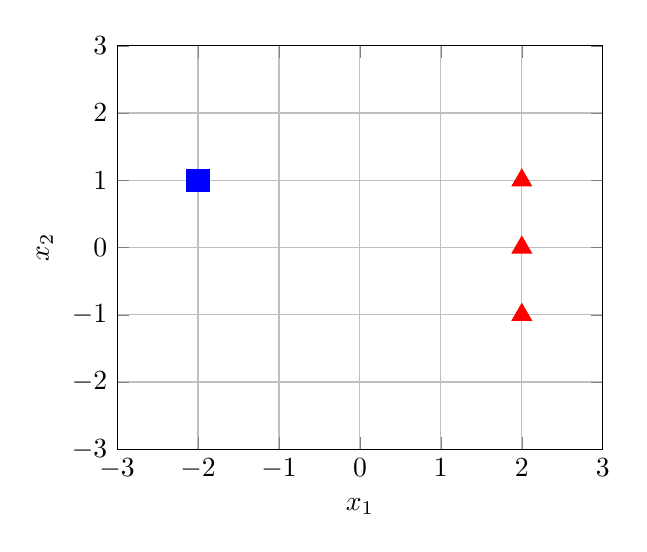
\begin{tikzpicture}
    \begin{axis}[
        scale=0.9, mark size=4.0pt,
        xmin=-3, xmax=3, xtick={-3,...,3},
        ymin=-3, ymax=3, ytick={-3,...,3},
        samples=50, grid=major, xlabel=$x_1$, ylabel=$x_2$]
        %\addplot[blue, ultra thick] (x,x*x);
        %\addplot[red,  ultra thick] (x*x,x);
        \addplot [
            scatter,
            only marks,
            point meta=explicit symbolic,
            scatter/classes={
                a={mark=square*,blue},
                b={mark=triangle*,red}
            },
            nodes near coords*={},
            visualization depends on={\thisrow{myvalue} \as \myvalue},
        ] table [meta=label] {
            x y label myvalue
            -2  1 a 1
            2 1 b 2
            2 0 b 3
            2 -1 b 4
        };
    \end{axis}
    \end{tikzpicture}
    \end{center}
    \caption{}
    \label{fig:percdata}
\end{figure}

\begin{subparts}

    \subpart[1] Suppose blue squares have $y = +1$ and red triangles have $y = -1$. Does the order in which Perceptron is presented with the training examples affect the final decision boundary?
    \begin{checkboxes}
     \choice Yes
     \choice No
     \choice It depends
    \end{checkboxes}
    \begin{soln}
    No. Regardless of the order, it will never make a mistake on the plus points, and it will always make a mistake on the minus point.
    \end{soln}
    \begin{qauthor}
    Matt
    \end{qauthor}
    
    \subpart[1] Now suppose we swap the labeling so that blue squares have $y = -1$ and red triangles have $y = +1$. Does the order in which Perceptron is presented with the training examples affect the final decision boundary? 
    \begin{checkboxes}
     \choice Yes
     \choice No
     \choice It depends
    \end{checkboxes}
    \begin{soln}
    Yes. Whichever minus point is presented first will lock in the decision boundary that correctly classifies all the other points.
    \end{soln}
    \begin{qauthor}
    Matt
    \end{qauthor}
    
    \subpart[1] According to the Perceptron Mistake Bound what is the upper bound on the number of mistakes that could be made on this dataset?
    \begin{tcolorbox}[fit,height=1cm, width=2cm, blank, borderline={1pt}{-2pt}, nobeforeafter]
        %solution
    \end{tcolorbox}
    \begin{soln}
    $(R/\gamma)^2 = (sqrt(1 + 4)/4)^2$
    \end{soln}
    \begin{qauthor}
    Matt
    \end{qauthor}
    
\end{subparts}
    

\part[2] What are the parameters after one \emph{more} epoch of gradient descent (i.e. two total epochs)?
    \begin{tcolorbox}[fit,height=1cm, width=15cm, blank, borderline={1pt}{-2pt}]
    %solution
    \end{tcolorbox}
    \begin{soln}
    Input solution here
    \end{soln}
    \begin{qauthor}
    Matt
    \end{qauthor}
    
\part[15] [Sana, Weyxin] You are performing a linear regression on a dataset that consists of $2m$ points and $m$ features. Your friend, Lucy, suggests using a closed-form solution to obtain your parameter estimates, $\hat{\theta}$. Another friend, Josh, suggests that stochastic gradient descent is a better approach. They get into a heated debate and turn to you to resolve it. You decide to pick a side based on analysis using a small subset of the data.
\begin{table}[H]
    \centering
        \begin{tabular}{llllll}
        $x_1$ & -1 & 0 & 1 & 2 \\
        $x_2$ & 1 & -1 & 1 & 1 \\
        $y$ & -1 & 0 & 1 & -1
        \end{tabular}
\end{table}
\begin{subparts}
    \subpart[5] Calculate the closed form solution for $\hat{\theta}$
    Assume there is no bias term and write inverse formula
    
    \begin{soln}
     $X^T X = \begin{bmatrix}
     -1 & 0 & 1 & 2\\
     1 & -1 & 1 & 1
     \end{bmatrix}
     \begin{bmatrix}
     -1 & 1\\
     0 & -1\\
     1 & 1\\
     2 & 1
     \end{bmatrix}
     = \begin{bmatrix}
     6 & 2\\
     2 & 4
     \end{bmatrix}$
     
     $(X^T X)^{-1} = \frac{1}{24-4}
     \begin{bmatrix}
     6 & 2\\
     2 & 4
     \end{bmatrix}
     = \begin{bmatrix}
     1/5 & -1/10\\
     -1/10 & 3/10
     \end{bmatrix}$
     
     $X^T Y = \begin{bmatrix}
     -1 & 0 & 1 & 2\\
     1 & -1 & 1 & 1
     \end{bmatrix}
     \begin{bmatrix}
     1 \\ 
     0\\
     1 \\
     -1
     \end{bmatrix}
     = \begin{bmatrix}
     0 \\
     1
     \end{bmatrix}$
     
     $(X^T X)^{-1}X^T Y = \hat{\theta} =
     \begin{bmatrix}
     1/5 & -1/10\\
     -1/10 & 3/10
     \end{bmatrix}
     \begin{bmatrix}
     0 \\
     1
     \end{bmatrix}
     = \boxed{\begin{bmatrix}
     1/10\\
     -3/10
     \end{bmatrix}}$
    \end{soln}
    
    \subpart[5] Calculate $\hat{\theta}$ for one pass of stochastic gradient descent, in the order of the points from the first to the last. Initialize $\wv = [0,0]^T$, $\eta = 1$, and assume there is no bias term.
    
    \begin{soln}
    $J(\wv; x^{(i)}; y^{(i)}) = (y^{(i)}-\wv^T x^{(i)})^2$\\[0.1 in]
    $\frac{\partial J(\wv; x^{(i)}; y^{(i)})}{w_k} = -2x_k^{(i)}(y^{(i)} - \wv^T x^{(i)}) = -2x_k^{(i)}(y^{(i)} - w_1x_1^{(i)} - w_2x_2^{(i)})$\\[0.1 in]
    $\nabla J(\wv, x^{(i)}; y^{(i)}) = \begin{bmatrix}
    \frac{\partial J(\wv; x^{(i)}; y^{(i)})}{w_1} \\
    \frac{\partial J(\wv; x^{(i)}; y^{(i)})}{w_2}
    \end{bmatrix} = \begin{bmatrix}
    -2x_1^{(i)}(y^{(i)} - w_1x_1^{(i)} - w_2x_2^{(i)}) \\
    -2x_2^{(i)}(y^{(i)} - w_1x_1^{(i)} - w_2x_2^{(i)})
    \end{bmatrix}$\\
    
    $(-1, 1, -1)$\\[0.05 in]
    $\wv = \begin{bmatrix}
    0 \\ 0
    \end{bmatrix} - 1 \begin{bmatrix}
    -2(-1)(-1-0-0) \\
    -2(1)(-1-0-0)
    \end{bmatrix} = \begin{bmatrix}
    0 \\ 0
    \end{bmatrix} - \begin{bmatrix}
    -2 \\ 2
    \end{bmatrix} = 
    \begin{bmatrix}
    2 \\ -2
    \end{bmatrix}$\\
    
    $(0, -1, 0)$\\[0.05 in]
    $\wv = \begin{bmatrix}
    2 \\ -2
    \end{bmatrix} - 1 \begin{bmatrix}
    -2(0)(0-0+2) \\
    -2(-1)(0-0+2)
    \end{bmatrix} = \begin{bmatrix}
    2 \\ -2
    \end{bmatrix} - \begin{bmatrix}
    0 \\ 4
    \end{bmatrix} = 
    \begin{bmatrix}
    2 \\ -6
    \end{bmatrix}$\\
    
    $(1,1,1)$\\[0.05 in]
    $\wv = \begin{bmatrix}
    2 \\ -6
    \end{bmatrix} - 1 \begin{bmatrix}
    -2(1)(1-2+6) \\
    -2(1)(1-2+6)
    \end{bmatrix} = \begin{bmatrix}
    2 \\ -6
    \end{bmatrix} - \begin{bmatrix}
    -10 \\ -10
    \end{bmatrix} = 
    \begin{bmatrix}
    12 \\ 4
    \end{bmatrix}$\\
    
    $(2, 1, -1)$\\[0.05 in]
    $\wv = \begin{bmatrix}
    12 \\ 4
    \end{bmatrix} - 1 \begin{bmatrix}
    -2(2)(-1-24-4) \\
    -2(1)(-1-24-4)
    \end{bmatrix} = \begin{bmatrix}
    12 \\ 4
    \end{bmatrix} - \begin{bmatrix}
    116 \\ 58
    \end{bmatrix} = \boxed{\begin{bmatrix}
    -104 \\ -54
    \end{bmatrix}}$
    \end{soln}

\end{subparts}

 \part[1] \textbf{True or False:} The number of parameters in a
    Perceptron grows linearly with the number of features ($M$) and
    logarithmically with the number of examples ($N$). %\textbf{Briefly justify your answer.}
    \begin{checkboxes}
     \choice True 
     \choice False
   \end{checkboxes}
   %\fillwithlines{6em}
    \begin{soln}
      False. The number of parameters is always $M$.
    \end{soln}
    \begin{qauthor}
      Matt
    \end{qauthor}

  % GOOD QUESTION, but redundant b/c Henry's KNN questions focus a lot on categorical features
\part[2] \textbf{Short Answer:} Consider a dataset with both
  continuous and categorical features. Could $k$-Nearest Neighbor be
  used to classify the data? If not, explain why not. If so, explain
  how you could compute the distance between two data points with both
  continuous and categorical features.
  \fillwithlines{6em}
   \begin{soln}
    Yes, you could. One example is, you could map the categorical features into continuous values in order to compute distance using a distance metric such as euclidean/manhattan.
  \end{soln}
  \begin{qauthor}
    Mukund
  \end{qauthor}

% Removed for time.
\part Suppose you are training a learner on some set of training examples. Determine whether online learning or batch learning is best suited for each scenario.

\begin{subparts}

    \subpart[1] Stock market prediction.
    \begin{checkboxes}
     \choice online learning
     \choice batch learning
    \end{checkboxes}
    \begin{soln}
    online learning
    \end{soln}
    \begin{qauthor}    Sami    \end{qauthor}
    
    \subpart[1] Cancer diagnosis prediction.
    \begin{checkboxes}
     \choice online learning
     \choice batch learning
    \end{checkboxes}
    \begin{soln}
    batch learning
    \end{soln}
    \begin{qauthor}    Sami    \end{qauthor}

\end{subparts}


\end{parts}